
%% bare_conf.tex
%% V1.3
%% 2007/01/11
%% by Michael Shell
%% See:
%% http://www.michaelshell.org/
%% for current contact information.
%%
%% This is a skeleton file demonstrating the use of IEEEtran.cls
%% (requires IEEEtran.cls version 1.7 or later) with an IEEE conference paper.
%%
%% Support sites:
%% http://www.michaelshell.org/tex/ieeetran/
%% http://www.ctan.org/tex-archive/macros/latex/contrib/IEEEtran/
%% and
%% http://www.ieee.org/

%%*************************************************************************
%% Legal Notice:
%% This code is offered as-is without any warranty either expressed or
%% implied; without even the implied warranty of MERCHANTABILITY or
%% FITNESS FOR A PARTICULAR PURPOSE! 
%% User assumes all risk.
%% In no event shall IEEE or any contributor to this code be liable for
%% any damages or losses, including, but not limited to, incidental,
%% consequential, or any other damages, resulting from the use or misuse
%% of any information contained here.
%%
%% All comments are the opinions of their respective authors and are not
%% necessarily endorsed by the IEEE.
%%
%% This work is distributed under the LaTeX Project Public License (LPPL)
%% ( http://www.latex-project.org/ ) version 1.3, and may be freely used,
%% distributed and modified. A copy of the LPPL, version 1.3, is included
%% in the base LaTeX documentation of all distributions of LaTeX released
%% 2003/12/01 or later.
%% Retain all contribution notices and credits.
%% ** Modified files should be clearly indicated as such, including  **
%% ** renaming them and changing author support contact information. **
%%
%% File list of work: IEEEtran.cls, IEEEtran_HOWTO.pdf, bare_adv.tex,
%%                    bare_conf.tex, bare_jrnl.tex, bare_jrnl_compsoc.tex
%%*************************************************************************

% *** Authors should verify (and, if needed, correct) their LaTeX system  ***
% *** with the testflow diagnostic prior to trusting their LaTeX platform ***
% *** with production work. IEEE's font choices can trigger bugs that do  ***
% *** not appear when using other class files.                            ***
% The testflow support page is at:
% http://www.michaelshell.org/tex/testflow/



% Note that the a4paper option is mainly intended so that authors in
% countries using A4 can easily print to A4 and see how their papers will
% look in print - the typesetting of the document will not typically be
% affected with changes in paper size (but the bottom and side margins will).
% Use the testflow package mentioned above to verify correct handling of
% both paper sizes by the user's LaTeX system.
%
% Also note that the "draftcls" or "draftclsnofoot", not "draft", option
% should be used if it is desired that the figures are to be displayed in
% draft mode.
%
\documentclass[10pt, conference, compsocconf]{IEEEtran}
% Add the compsocconf option for Computer Society conferences.
%
% If IEEEtran.cls has not been installed into the LaTeX system files,
% manually specify the path to it like:
% \documentclass[conference]{../sty/IEEEtran}

\usepackage{algorithm}
\usepackage{algorithmic}

\usepackage{amssymb}
\usepackage{amsmath}
%\usepackage{subfigure}
\setcounter{tocdepth}{3}
\usepackage{graphicx}
\usepackage{enumerate}
\usepackage{verbatim}




% Some very useful LaTeX packages include:
% (uncomment the ones you want to load)


% *** MISC UTILITY PACKAGES ***
%
%\usepackage{ifpdf}
% Heiko Oberdiek's ifpdf.sty is very useful if you need conditional
% compilation based on whether the output is pdf or dvi.
% usage:
% \ifpdf
%   % pdf code
% \else
%   % dvi code
% \fi
% The latest version of ifpdf.sty can be obtained from:
% http://www.ctan.org/tex-archive/macros/latex/contrib/oberdiek/
% Also, note that IEEEtran.cls V1.7 and later provides a builtin
% \ifCLASSINFOpdf conditional that works the same way.
% When switching from latex to pdflatex and vice-versa, the compiler may
% have to be run twice to clear warning/error messages.






% *** CITATION PACKAGES ***
%
%\usepackage{cite}
% cite.sty was written by Donald Arseneau
% V1.6 and later of IEEEtran pre-defines the format of the cite.sty package
% \cite{} output to follow that of IEEE. Loading the cite package will
% result in citation numbers being automatically sorted and properly
% "compressed/ranged". e.g., [1], [9], [2], [7], [5], [6] without using
% cite.sty will become [1], [2], [5]--[7], [9] using cite.sty. cite.sty's
% \cite will automatically add leading space, if needed. Use cite.sty's
% noadjust option (cite.sty V3.8 and later) if you want to turn this off.
% cite.sty is already installed on most LaTeX systems. Be sure and use
% version 4.0 (2003-05-27) and later if using hyperref.sty. cite.sty does
% not currently provide for hyperlinked citations.
% The latest version can be obtained at:
% http://www.ctan.org/tex-archive/macros/latex/contrib/cite/
% The documentation is contained in the cite.sty file itself.






% *** GRAPHICS RELATED PACKAGES ***
%
\ifCLASSINFOpdf
  % \usepackage[pdftex]{graphicx}
  % declare the path(s) where your graphic files are
  % \graphicspath{{../pdf/}{../jpeg/}}
  % and their extensions so you won't have to specify these with
  % every instance of \includegraphics
  % \DeclareGraphicsExtensions{.pdf,.jpeg,.png}
\else
  % or other class option (dvipsone, dvipdf, if not using dvips). graphicx
  % will default to the driver specified in the system graphics.cfg if no
  % driver is specified.
  % \usepackage[dvips]{graphicx}
  % declare the path(s) where your graphic files are
  % \graphicspath{{../eps/}}
  % and their extensions so you won't have to specify these with
  % every instance of \includegraphics
  % \DeclareGraphicsExtensions{.eps}
\fi
% graphicx was written by David Carlisle and Sebastian Rahtz. It is
% required if you want graphics, photos, etc. graphicx.sty is already
% installed on most LaTeX systems. The latest version and documentation can
% be obtained at: 
% http://www.ctan.org/tex-archive/macros/latex/required/graphics/
% Another good source of documentation is "Using Imported Graphics in
% LaTeX2e" by Keith Reckdahl which can be found as epslatex.ps or
% epslatex.pdf at: http://www.ctan.org/tex-archive/info/
%
% latex, and pdflatex in dvi mode, support graphics in encapsulated
% postscript (.eps) format. pdflatex in pdf mode supports graphics
% in .pdf, .jpeg, .png and .mps (metapost) formats. Users should ensure
% that all non-photo figures use a vector format (.eps, .pdf, .mps) and
% not a bitmapped formats (.jpeg, .png). IEEE frowns on bitmapped formats
% which can result in "jaggedy"/blurry rendering of lines and letters as
% well as large increases in file sizes.
%
% You can find documentation about the pdfTeX application at:
% http://www.tug.org/applications/pdftex





% *** MATH PACKAGES ***
%
%\usepackage[cmex10]{amsmath}
% A popular package from the American Mathematical Society that provides
% many useful and powerful commands for dealing with mathematics. If using
% it, be sure to load this package with the cmex10 option to ensure that
% only type 1 fonts will utilized at all point sizes. Without this option,
% it is possible that some math symbols, particularly those within
% footnotes, will be rendered in bitmap form which will result in a
% document that can not be IEEE Xplore compliant!
%
% Also, note that the amsmath package sets \interdisplaylinepenalty to 10000
% thus preventing page breaks from occurring within multiline equations. Use:
%\interdisplaylinepenalty=2500
% after loading amsmath to restore such page breaks as IEEEtran.cls normally
% does. amsmath.sty is already installed on most LaTeX systems. The latest
% version and documentation can be obtained at:
% http://www.ctan.org/tex-archive/macros/latex/required/amslatex/math/





% *** SPECIALIZED LIST PACKAGES ***
%
%\usepackage{algorithmic}
% algorithmic.sty was written by Peter Williams and Rogerio Brito.
% This package provides an algorithmic environment fo describing algorithms.
% You can use the algorithmic environment in-text or within a figure
% environment to provide for a floating algorithm. Do NOT use the algorithm
% floating environment provided by algorithm.sty (by the same authors) or
% algorithm2e.sty (by Christophe Fiorio) as IEEE does not use dedicated
% algorithm float types and packages that provide these will not provide
% correct IEEE style captions. The latest version and documentation of
% algorithmic.sty can be obtained at:
% http://www.ctan.org/tex-archive/macros/latex/contrib/algorithms/
% There is also a support site at:
% http://algorithms.berlios.de/index.html
% Also of interest may be the (relatively newer and more customizable)
% algorithmicx.sty package by Szasz Janos:
% http://www.ctan.org/tex-archive/macros/latex/contrib/algorithmicx/




% *** ALIGNMENT PACKAGES ***
%
%\usepackage{array}
% Frank Mittelbach's and David Carlisle's array.sty patches and improves
% the standard LaTeX2e array and tabular environments to provide better
% appearance and additional user controls. As the default LaTeX2e table
% generation code is lacking to the point of almost being broken with
% respect to the quality of the end results, all users are strongly
% advised to use an enhanced (at the very least that provided by array.sty)
% set of table tools. array.sty is already installed on most systems. The
% latest version and documentation can be obtained at:
% http://www.ctan.org/tex-archive/macros/latex/required/tools/


%\usepackage{mdwmath}
%\usepackage{mdwtab}
% Also highly recommended is Mark Wooding's extremely powerful MDW tools,
% especially mdwmath.sty and mdwtab.sty which are used to format equations
% and tables, respectively. The MDWtools set is already installed on most
% LaTeX systems. The lastest version and documentation is available at:
% http://www.ctan.org/tex-archive/macros/latex/contrib/mdwtools/


% IEEEtran contains the IEEEeqnarray family of commands that can be used to
% generate multiline equations as well as matrices, tables, etc., of high
% quality.


%\usepackage{eqparbox}
% Also of notable interest is Scott Pakin's eqparbox package for creating
% (automatically sized) equal width boxes - aka "natural width parboxes".
% Available at:
% http://www.ctan.org/tex-archive/macros/latex/contrib/eqparbox/





% *** SUBFIGURE PACKAGES ***
%\usepackage[tight,footnotesize]{subfigure}
% subfigure.sty was written by Steven Douglas Cochran. This package makes it
% easy to put subfigures in your figures. e.g., "Figure 1a and 1b". For IEEE
% work, it is a good idea to load it with the tight package option to reduce
% the amount of white space around the subfigures. subfigure.sty is already
% installed on most LaTeX systems. The latest version and documentation can
% be obtained at:
% http://www.ctan.org/tex-archive/obsolete/macros/latex/contrib/subfigure/
% subfigure.sty has been superceeded by subfig.sty.



%\usepackage[caption=false]{caption}
%\usepackage[font=footnotesize]{subfig}
% subfig.sty, also written by Steven Douglas Cochran, is the modern
% replacement for subfigure.sty. However, subfig.sty requires and
% automatically loads Axel Sommerfeldt's caption.sty which will override
% IEEEtran.cls handling of captions and this will result in nonIEEE style
% figure/table captions. To prevent this problem, be sure and preload
% caption.sty with its "caption=false" package option. This is will preserve
% IEEEtran.cls handing of captions. Version 1.3 (2005/06/28) and later 
% (recommended due to many improvements over 1.2) of subfig.sty supports
% the caption=false option directly:
%\usepackage[caption=false,font=footnotesize]{subfig}
%
% The latest version and documentation can be obtained at:
% http://www.ctan.org/tex-archive/macros/latex/contrib/subfig/
% The latest version and documentation of caption.sty can be obtained at:
% http://www.ctan.org/tex-archive/macros/latex/contrib/caption/




% *** FLOAT PACKAGES ***
%
%\usepackage{fixltx2e}
% fixltx2e, the successor to the earlier fix2col.sty, was written by
% Frank Mittelbach and David Carlisle. This package corrects a few problems
% in the LaTeX2e kernel, the most notable of which is that in current
% LaTeX2e releases, the ordering of single and double column floats is not
% guaranteed to be preserved. Thus, an unpatched LaTeX2e can allow a
% single column figure to be placed prior to an earlier double column
% figure. The latest version and documentation can be found at:
% http://www.ctan.org/tex-archive/macros/latex/base/



%\usepackage{stfloats}
% stfloats.sty was written by Sigitas Tolusis. This package gives LaTeX2e
% the ability to do double column floats at the bottom of the page as well
% as the top. (e.g., "\begin{figure*}[!b]" is not normally possible in
% LaTeX2e). It also provides a command:
%\fnbelowfloat
% to enable the placement of footnotes below bottom floats (the standard
% LaTeX2e kernel puts them above bottom floats). This is an invasive package
% which rewrites many portions of the LaTeX2e float routines. It may not work
% with other packages that modify the LaTeX2e float routines. The latest
% version and documentation can be obtained at:
% http://www.ctan.org/tex-archive/macros/latex/contrib/sttools/
% Documentation is contained in the stfloats.sty comments as well as in the
% presfull.pdf file. Do not use the stfloats baselinefloat ability as IEEE
% does not allow \baselineskip to stretch. Authors submitting work to the
% IEEE should note that IEEE rarely uses double column equations and
% that authors should try to avoid such use. Do not be tempted to use the
% cuted.sty or midfloat.sty packages (also by Sigitas Tolusis) as IEEE does
% not format its papers in such ways.





% *** PDF, URL AND HYPERLINK PACKAGES ***
%
%\usepackage{url}
% url.sty was written by Donald Arseneau. It provides better support for
% handling and breaking URLs. url.sty is already installed on most LaTeX
% systems. The latest version can be obtained at:
% http://www.ctan.org/tex-archive/macros/latex/contrib/misc/
% Read the url.sty source comments for usage information. Basically,
% \url{my_url_here}.





% *** Do not adjust lengths that control margins, column widths, etc. ***
% *** Do not use packages that alter fonts (such as pslatex).         ***
% There should be no need to do such things with IEEEtran.cls V1.6 and later.
% (Unless specifically asked to do so by the journal or conference you plan
% to submit to, of course. )


% correct bad hyphenation here
\hyphenation{op-tical net-works semi-conduc-tor}


\begin{document}
%
% paper title
% can use linebreaks \\ within to get better formatting as desired
\title{A Navigation Algorithm Inspired by Human Navigation}


% author names and affiliations
% use a multiple column layout for up to two different
% affiliations

\author{

\IEEEauthorblockN{Vijesh M}
\IEEEauthorblockA{Student, PESIT, Bangalore, India\\
Intern, ISI, Chennai, India\\
mv.vijesh@gmail.com}

\and

\IEEEauthorblockN{Sudarshan Iyengar}
\IEEEauthorblockA{ISI\\
Chennai, India\\
sudarshaniisc@gmail.com}

\and

\IEEEauthorblockN{Vijay Mahantesh SM}
\IEEEauthorblockA{Student, PESIT, Bangalore, India\\
Intern, ISI, Chennai, India\\
vijaym123@gmail.com}

\and

\IEEEauthorblockN{Amitash Ramesh}
\IEEEauthorblockA{Student, DSCE, Bangalore, India\\
Intern, ISI, Chennai, India\\
amitashr@gmail.com}

\and

\IEEEauthorblockN{C Pandurangan}
\IEEEauthorblockA{ISI\\
Chennai, India\\
prangan55@gmail.com}

\and

\IEEEauthorblockN{Veni Madhavan}
\IEEEauthorblockA{Computer Science and Automation\\
Indian Institute of Science\\
Bangalore, India}
}

% conference papers do not typically use \thanks and this command
% is locked out in conference mode. If really needed, such as for
% the acknowledgment of grants, issue a \IEEEoverridecommandlockouts
% after \documentclass

% for over three affiliations, or if they all won't fit within the width
% of the page, use this alternative format:
% 
%\author{\IEEEauthorblockN{Michael Shell\IEEEauthorrefmark{1},
%Homer Simpson\IEEEauthorrefmark{2},
%James Kirk\IEEEauthorrefmark{3}, 
%Montgomery Scott\IEEEauthorrefmark{3} and
%Eldon Tyrell\IEEEauthorrefmark{4}}
%\IEEEauthorblockA{\IEEEauthorrefmark{1}School of Electrical and Computer Engineering\\
%Georgia Institute of Technology,
%Atlanta, Georgia 30332--0250\\ Email: see http://www.michaelshell.org/contact.html}
%\IEEEauthorblockA{\IEEEauthorrefmark{2}Twentieth Century Fox, Springfield, USA\\
%Email: homer@thesimpsons.com}
%\IEEEauthorblockA{\IEEEauthorrefmark{3}Starfleet Academy, San Francisco, California 96678-2391\\
%Telephone: (800) 555--1212, Fax: (888) 555--1212}
%\IEEEauthorblockA{\IEEEauthorrefmark{4}Tyrell Inc., 123 Replicant Street, Los Angeles, California 90210--4321}}


% use for special paper notices
%\IEEEspecialpapernotice{(Invited Paper)}


% make the title area
\maketitle


\begin{abstract}
Human navigation has been a topic of interest in spatial cognition from the past few decades. It has been experimentally observed that humans accomplish the task of way-finding a destination in an unknown environment by recognizing landmarks. Investigations using network analytic techniques reveal that humans, when asked to way-find their destination, learn the top ranked nodes of a network.  In this paper we report a study simulating the strategy used by humans to recognize the centers of a network. We show that 
the paths obtained from our simulation has the same properties as the paths obtained in human based experiment. The simulation thus performed leads to a novel way of path-finding in a network. We discuss the performance of our method and compare it with the existing techniques to find a path between a pair of nodes in a network. 
\end{abstract}

\begin{IEEEkeywords}
search algorithm; human navigation; hotspots, path concatenation, center strategic paths;
\end{IEEEkeywords}


% For peer review papers, you can put extra information on the cover
% page as needed:
% \ifCLASSOPTIONpeerreview
% \begin{center} \bfseries EDICS Category: 3-BBND \end{center}
% \fi
%
% For peerreview papers, this IEEEtran command inserts a page break and
% creates the second title. It will be ignored for other modes.
\IEEEpeerreviewmaketitle



\section{Introduction}
% no \IEEEPARstart
The problem of finding a target vertex in a network where one is provided with just the local information is a well studied problem. Starting from the work of Milgram in 1967~\cite{milgram67}, the current methods include routing using full-tables~\cite{gavoille01}, interval routing~\cite{gavoille99,gavoille01}, 
%routing labeling schemes~\cite{peleg00,thorup01}, 
greedy routing~\cite{giordano01,kleinberg-1-00}, geographic routing~\cite{giordano01}, compass routing~\cite{giordano01}, etc., These routing techniques are mainly used in transportation networks and in wired as well as wireless communication networks. For detailed survey one can refer to~\cite{gavoille99, gavoille01, giordano01}. %and~\cite{peleg00}
   For surveys of the routing methods in social networks and email networks in particular, one is referred to%~\cite{adamic02, adamic01, fraigniaud07, kleinberg-1-00, nowell05}\\
~\cite{adamic02, adamic01, kleinberg-1-00}.\\
%
%(adamic02)[3]
%(adamic01)[4]
%(fraigniaud07)[33]
%(gavoille99)[37]
%(gavoille01)[38]
%(giordano01)[43]
%(kleinberg-1-00)[47]
%(nowell05)[54]
%(peleg00)[56]
%(thorup01)[65]
 
In the classical small world experiment by Milgram~\cite{milgram67}, the letter from Nebraska was to reach Boston. This is a scenario where the sender actively needs to participate in the process of helping the letter reach the destination, while the receiver remains passive. 
% Let us  consider a variation of this problem where both sender and receiver participate in the process of finding a path between them.
\\
%\newpage
{\bf Motivation}

Sudarshan et al., in \cite{sudarshan11} presents a network analytic approach to understand human navigation. Their experiment comprises of making human participants navigate on a network that is unknown to them. 
%Participants are given a source node and are asked to navigate to a destination node. 
At any instance, participant can view the adjacent nodes of the node that s/he is currently present. Several 
%such 
source-destination node pairs are given to the participant. 
%The time taken and the path taken are recorded. They observe that participants eventually learn a strategy which helps them navigate easily and quickly. 
They show that the participants learn a few landmark nodes which they use as via media to navigate. 
%They further show that these landmark nodes have superior closeness-centrality ranking.\\
The strategy of human participants in the above mentioned experiment to learn centers of a network and the pursuit of paths through the centers has motivated the proposal of this novel navigation algorithm.\\

{\bf The Technique}

In an unweighted graph $G(V,E)$, given a source vertex $s$ and a destination vertex $t$, a straight forward approach to establish a path between $s$ and $t$ is to take a random walk from $s$ till we reach $t$. One way to better this random walk method is to take a two way random walk, one from the source $s$ and the other from the destination $t$ and stop once the two random walks intersect. This method is expected to be quicker than the first in terms of number of hops that is required to establish a path. We provide 
empirical results to support this.\\

We describe our algorithm (\emph{path concatenation algorithm} or PCA) and compare it with two other path finding strategies based on random walks. We apply PCA on various synthetic networks and discuss its performance. We show that PCA yields center-strategic paths on scale free networks - as was the  case with the paths that the participants took in the two experiments.\\

\section{Related Work}
\label{sec:4_related_work}

Kleinberg's work~\cite{kleinberg-2-00} on navigation in a small world, highlighted the fact that it is easier to find short chains between points in \emph{some} networks than \emph{others}. Adamic et al., in~\cite{adamic01} introduced several local search strategies to find a path to the given destination vertex.\\
%In~\cite{kim02}, Kim et al., numerically compares the local path finding strategies with that of global path finding strategies on scale free networks.\\

A rigorous graph theory based approach to path finding strategy was proposed 
by Gavoille et al.,~\cite{gavoille04}. They provide a method of navigation based on vertex labeling. The established labeling strategy allows one to compute the distance between any two vertices directly.
% They establish a labeling strategy for the vertices of a graph in a way that allows one to compute the distance between any two vertices directly from the labels, without using any additional information about the network.\\
% Adamic et al., in~\cite{adamic05} addresses the question of how participants in a small world experiment are able to find short paths in a social network using only local information about their immediate contacts.\\
A detailed survey on decentralized search algorithms on networks that exhibit small-world phenomena is given by Kleinberg in~\cite{kleinberg06}.\\

Ozgur et al.,~\cite{simsek08} proposes a navigational technique based on a hybridized method of using degree and homophilly. 
%of vertices that yield better results than the currently known techniques.\\
Cajueiro et al., in~\cite{cajueiro09} proposed a learning framework based on a First-Visit Monte Carlo Algorithm. They show that the \emph{navigation difficulty} and \emph{learning velocity} are strongly related to the network topology.\\

Recently a novel method of navigating a network using the underlying spanning tree was proposed by Dragan et al. in~\cite{dragan11}. 
%The paper provides a thorough graph theoretic treatment of the navigation problem. 
They reduce the navigation problem on a graph $G$ to that of the underlying spanning tree and navigate on the latter.\\

On the application front, such navigational techniques are useful in a problem of finding paths between vertices in peer-to-peer systems. Crespo et al.,~\cite{crespo02} in their work on routing indices on Peer-to-Peer systems, propose a novel method of query forwarding from vertices to their neighbors that are more likely to have answers. They provide different novel routing schemes and evaluate their performance.\\

\section{Notations and Notions} 
\label{sec:4_notions}

A graph $G=(V,E)$ is composed of a set of nodes $V$ and a set of edges  $E$, with $|V|=n$ and $|E|=m$. Two nodes are said to be {\it connected} if there exists a path between them. The {\it distance} $d(v_1, v_2)$ between any two nodes is defined as the length of a shortest path between them, or set to $\infty$ if there exists no path between them. Given $v \in V$, $N_{G}(v)$ denotes the set of all adjacent vertices of $v$. Let $W_u=(u=v_0,v_1,v_2,....)$ denote a random walk starting from the vertex $u$. By $W_u[i]$ we mean the vertex at the $i$th step of the random walk $W_u$. e.g. $W_u[2]=v_2$. Let $T(W_u,i)$ denote the set $T(W_u,i)=\{v_0,v_1,...,v_i\}$ of all vertices that are being visited by the random walk $W_u$ during the first $i$ steps.\\

A {\it centrality index} is a real-valued function $C: V \rightarrow \mathbb R$ on the nodes. %~\cite{Brandes05}
The intuition is that the higher the value of this function, the more central this node is for the network. There are various indices; in this article we use the so-called {\it closeness centrality} \cite{Sabidussi66} $C_C(v)$, which is defined as the reciprocal of sum of the distances of $v$ to all other nodes. For any given graph, a centrality index can be used to define a ranking on the nodes, by sorting the nodes non-decreasingly by their centrality value. Ties if any, are broken arbitrarily. we denote the rank of a vertex by $R(v)$.Throughout the paper, we assume that the graph is an undirected simple graph, unless otherwise stated.\\

\section{The Algorithm}
\label{sec:idea}
The path concatenation algorithm is split into two components: The Learning Phase and The Navigation Phase.\\

The learning phase deals with the preprocessing of the graph G. Once the preprocessing phase is complete, the navigation phase describes how one can find a path between a given pair of vertices. 

\subsection{Learning Phase}
\label{sec:4_learning_phase}

Let $G_d$ be a distinct graph with vertex set $V$ and edge set $E_d$. $E_d$ is the directed edge set formed by splitting each edge in $E$ into two directional components. The learning phase involves updating the directed graph $G_d$, based on the random walks taken on $G$. Let $u,v\in_r V$ be two randomly picked vertices. Consider the random walks $W_u$ and $W_v$. As defined above, let $W_u=(W_u[0],W_u[1],...)$ and $W_v=(W_v[0],W_v[1],...)$.\\

Consider least $i$ such that $T(W_u,i)\cap T(W_v,i)\neq \emptyset$. Such an $i$ guarantees a vertex $h\in T(W_u,i)\cap T(W_v,i)$. Clearly, one can construct a path from $u$ to $h$ and another path from $v$ to $h$. Let us call these directed paths $P_{u,h}$ and $P_{v,h}$ respectively. Let $l(P_{u,h})$ and $l(P_{v,h})$ denote the respective path lengths.\\

We define two reward functions on $V$ and $E_d$ as follows:\\
%\emph{Vertex Reward} and \emph{Edge Reward} on the vertex set and the edge set respectively.\\

\subsubsection{Vertex Reward}

Consider a function $flag :V\rightarrow \mathbb{Z}$, where 
$flag(v)=0, \forall v\in V$ to begin with. In an iteration, we 
pick a random pair of vertices $u$ and $v$, and take random walks 
$W_u$ and $W_v$. Once the walks intersect at a vertex, say $h$, we 
increment $flag(h)$ by 1, i.e. $flag(h)=flag(h)+1$.\\

\subsubsection{Edge Reward}

Given the graph $G(V,E)$, at the end of the learning phase, we need 
to obtain a weighted directed graph $G(V,E_d)$. We define a reward function $R:E_d\rightarrow \mathbb{R}$. We first initialize $R(u,v)=0, \forall (u,v) \in E_d$. For every edge $(a,b)$ belonging to the path $P_{u,h}$, we increment the reward of that edge by $R(a,b)=R(a,b)+\frac{1}{l(P_{u,h})}$. 
A similar action is performed for all edges along the path $P_{v,h}$.
%Similarly for all edges $(c,d)$ belonging to the path $P_{v,h}$, we increment the reward of the edge $(c,d)$ by $R(c,d)=R(c,d)+\frac{1}{l(P_{v,h})}$.
Algorithm~\ref{4_learning_algorithm} depicts the pidgin code of the algorithm for the Learning Phase.\\

\begin{algorithm}
\label{4_learning_algorithm}
\caption{The Learning phase}
\begin{algorithmic}[1]
\renewcommand{\algorithmicrequire}{\textbf{Input:}}
\renewcommand{\algorithmicensure}{\textbf{Output:}}

\REQUIRE $G(V,E)$, $\alpha$
\ENSURE  $G_d(V,E_d)$, $R$

\STATE $R(a,b)\longleftarrow 0, \forall (a,b)\in E_d$

\STATE $flag(v)\longleftarrow 0, \forall v\in V$

\FORALL{$ (u,v) \in V\times V$}
\STATE 
\begin{itemize}
\renewcommand{\labelitemi}{$\bullet $}
\item Take random walks $W_u=(W_u[0],W_u[1],...W_u[i])$ and $W_v=(W_v[0],W_v[1],...W_v[i])$ until $T(W_u,i)$ $\bigcap$ $T(W_v,i)$ $\neq \emptyset$. \item Pick $h \in T(W_u,i)$ $\bigcap$ $T(W_v,i)$ \\
Compute $P_{u,h}$ and $P_{v,h}$\\
\item 
$l(P_{u,h})$ $\longleftarrow$ path length of $P_{u,h}$\\
$l(P_{v,h})$ $\longleftarrow$ path length of $P_{v,h}$


\item $flag(h) \longleftarrow flag(h)+1$

\item \textbf{for} every directed edge $(a,b) \in P_{u,h} $ \textbf{do}\\
\hspace{0.3 in} $R(a,b) \longleftarrow R(a,b) + \frac{1}{l(u,h)}$

\item \textbf{for} every directed edge $(c,d) \in P_{v,h} $ \textbf{do}\\
\hspace{0.3 in} $R(c,d) \longleftarrow R(c,d) + \frac{1}{l(v,h)}$

\end{itemize} 
\ENDFOR

\STATE Let $HotSpotOrdering \longleftarrow$ list of vertices in descending order of their $flag$ values (with ties arbitrarily broken).

\STATE Let the first $\alpha$ number of vertices from $HotSpotOrdering$ constitute the $HotSpots$ set. 

\STATE Compute and store the shortest paths between all pairs of vertices in the $HotSpot$ set. Given $u,v\in HotSpots$, $HotSpotLookup(u,v)$ returns a shortest path from $u$ to $v$.
\end{algorithmic}

\end{algorithm}

Figure.~\ref{4_learning_phase_diag} illustrates the learning phase of Algorithm \ref{4_learning_algorithm}. $u$ and $v$ are the chosen pair of vertices. The red walk from $u$ and the green walk from $v$ indicate the random walks $W_u$ and $W_v$ respectively. $h$ is the vertex at which the intersection has occurred. The blue path from $u$ and the pink path from $v$ indicate $P_{u,h}$ and $P_{v,h}$ respectively. $l(P_{u,h})$ and $l(P_{v,h})$ are the lengths of the blue and pink path respectively. The directed edges along the blue path and the pink path are rewarded with $\frac{1}{l(P_{u,h})}$ and $\frac{1}{l(P_{v,h})}$ respectively. $flag(h)$ is incremented by 1.\\

\begin{figure}[htp]
\centering
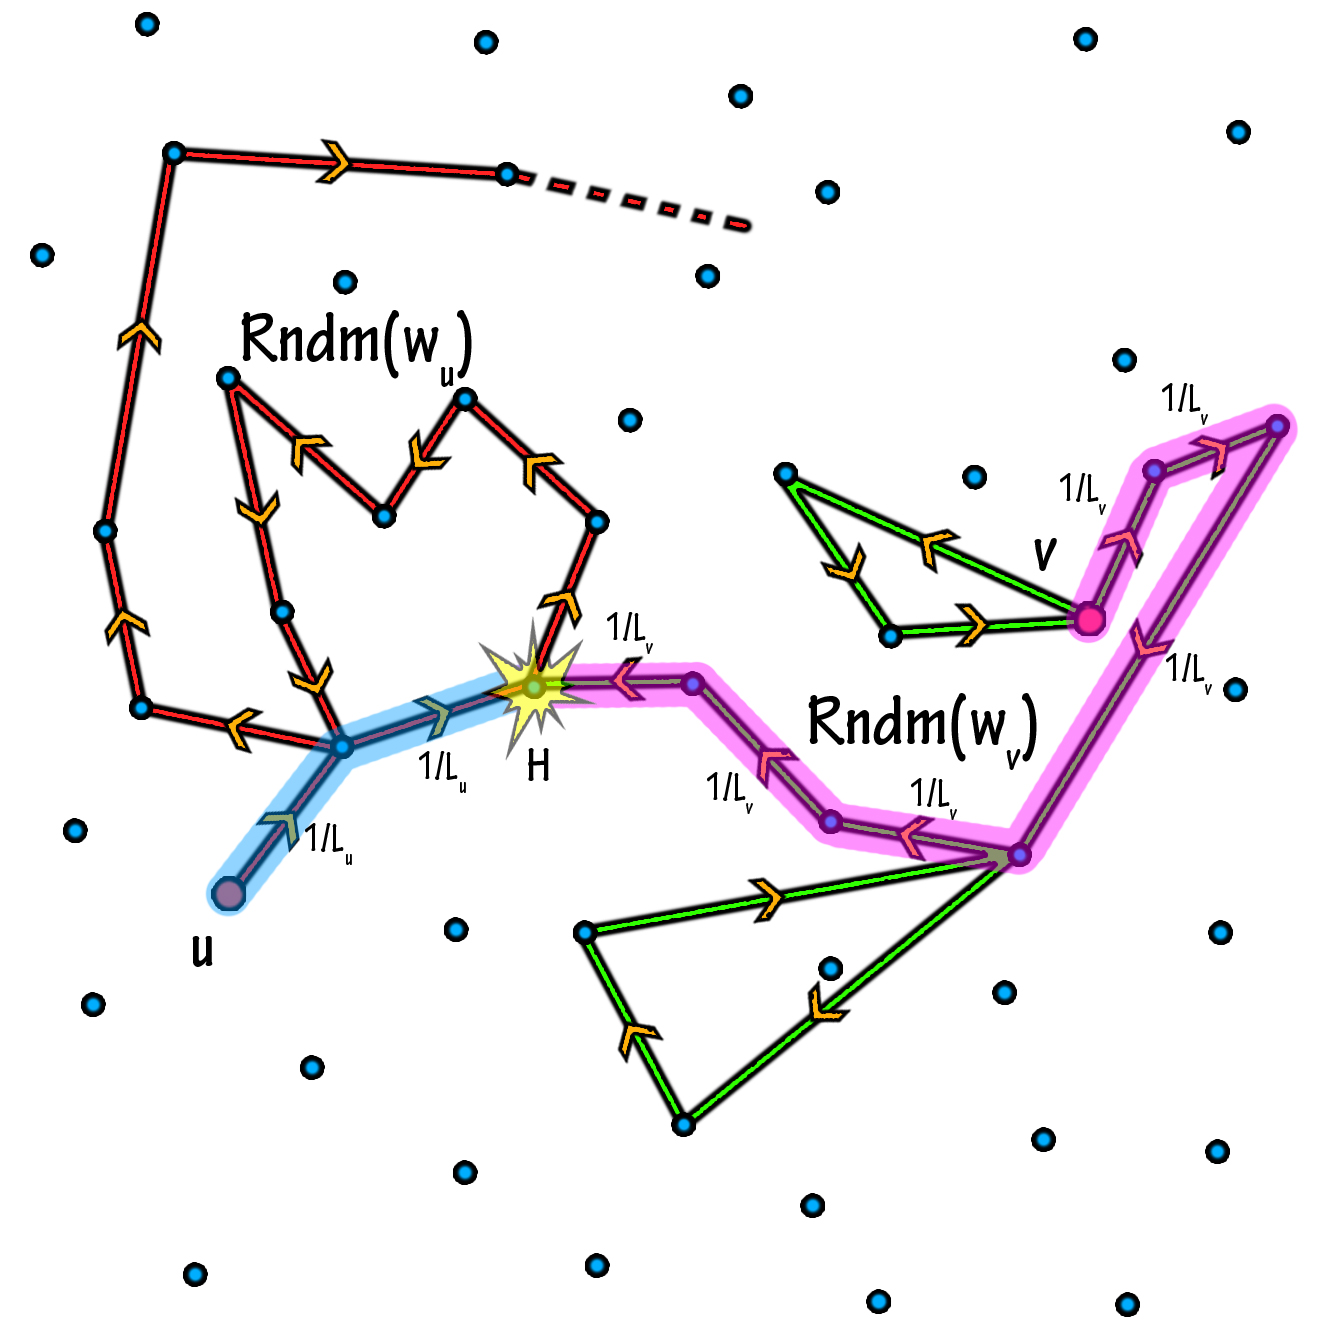
\includegraphics[scale=0.13]{Results/LearningComponent.jpg}
\caption{The Learning Phase}
\label{4_learning_phase_diag}
\end{figure}

%We now describe how one can find a path from a given source vertex $s$ to a destination vertex $t$ by making use of $HotSpotLookup$ and the weights in the directed weighted graph thus obtained.\\

\subsection{Navigation Phase}
\label{sec:4_navigation_phase}

The navigation phase makes use of the reward functions $flag$ and $R$ to find a path between a given source and destination. Both these information are embedded in $G_d(V,E_d)$. 
%output $G_d(V,E_d)$ and the set $R$, which contains the weights of the edges obtained in the learning phase to find a path between a given source vertex $s\in V$ to a destination vertex $t \in V$. 
The technique involves 3 stages:

\begin{enumerate}
\item Finding a path from $s$ to $h_s$, where $h_s\in HotSpots$
\item Finding a path from $t$ to $h_t$, where $h_t \in HotSpots$
\item Concatenating the paths $s$ to $h_s$, $h_s$ to $h_t$ and $h_t$ to $t$.
\end{enumerate}

The paths $s$ to $h_s$ and $t$ to $h_t$ are constructed by successively choosing edges with the highest weight. We call this the \emph{greedy traversal technique}. This is illustrated in Figure~\ref{4_greedy_traversal}. The paths thus obtained are finally concatenated to get a path from $s$ to $t$. See Figure~\ref{4_navigation_phase} for illustration.

\begin{figure}[htp]
\centering
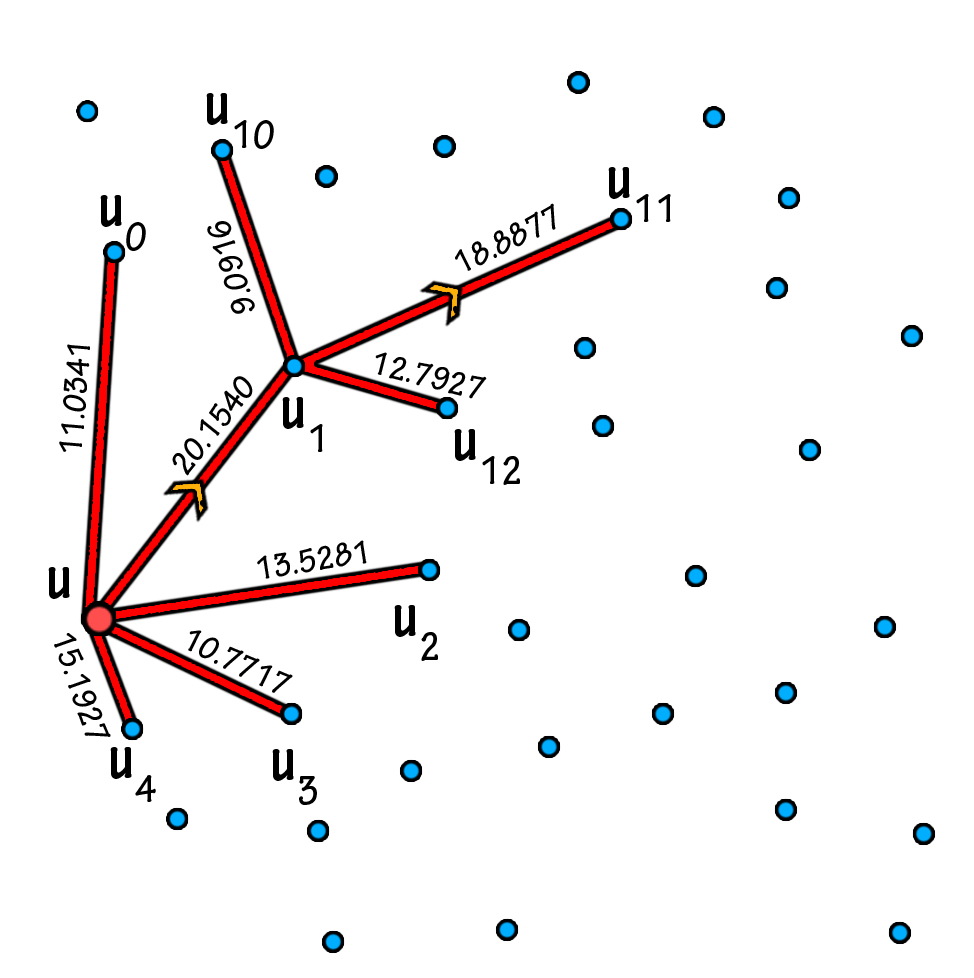
\includegraphics[scale=0.17]{Results/greedynavigation.jpg}
\caption{Greedy Traversal Technique}
\label{4_greedy_traversal}
\end{figure}

\begin{figure}[htp]
\centering
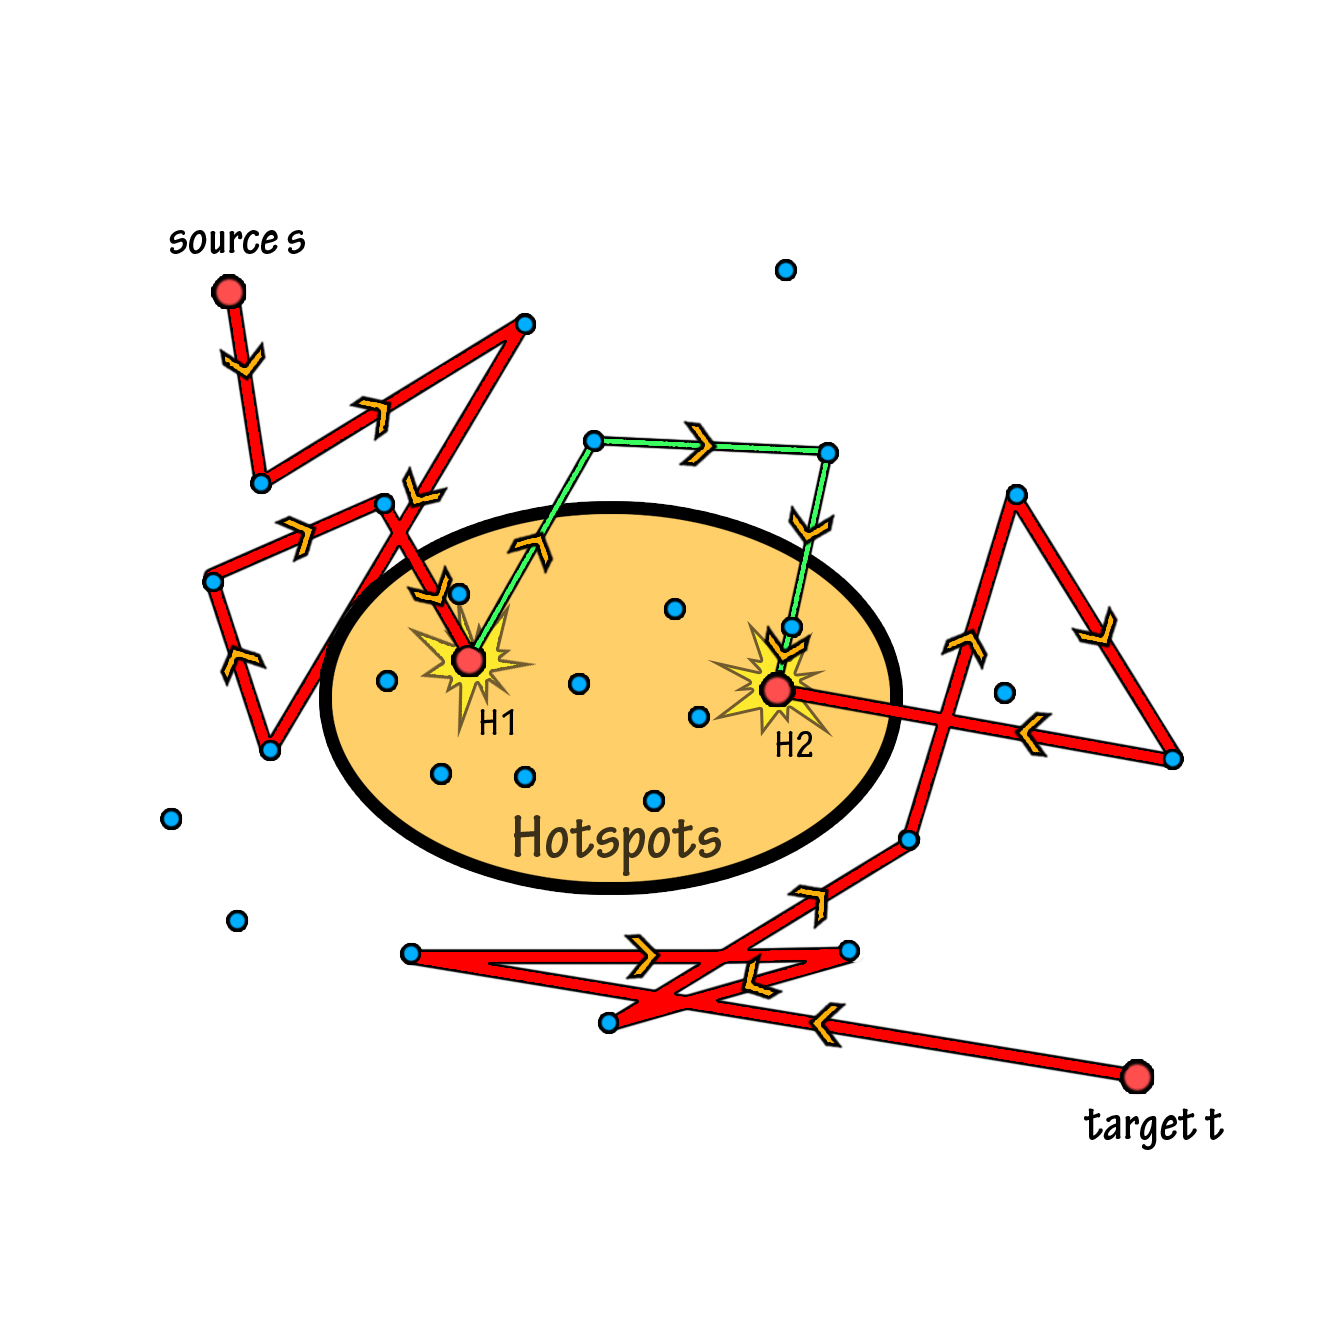
\includegraphics[scale=0.15]{Results/greedywalk.jpg}
\caption{The Navigation Phase}
\label{4_navigation_phase}
\end{figure}

\section{\label{4_results}Results and Discussions}

We discuss in this section, the results that were obtained when PCA was applied to several classes of graphs. We mainly test our algorithm on two types of synthetic networks: Barabasi-Albert graphs~\cite{barabasi02} and Erdos-Renyi graphs~\cite{erdos60}.\\

\subsection{Selection of optimum value of $\alpha$}

\begin{figure}[h]
\centering
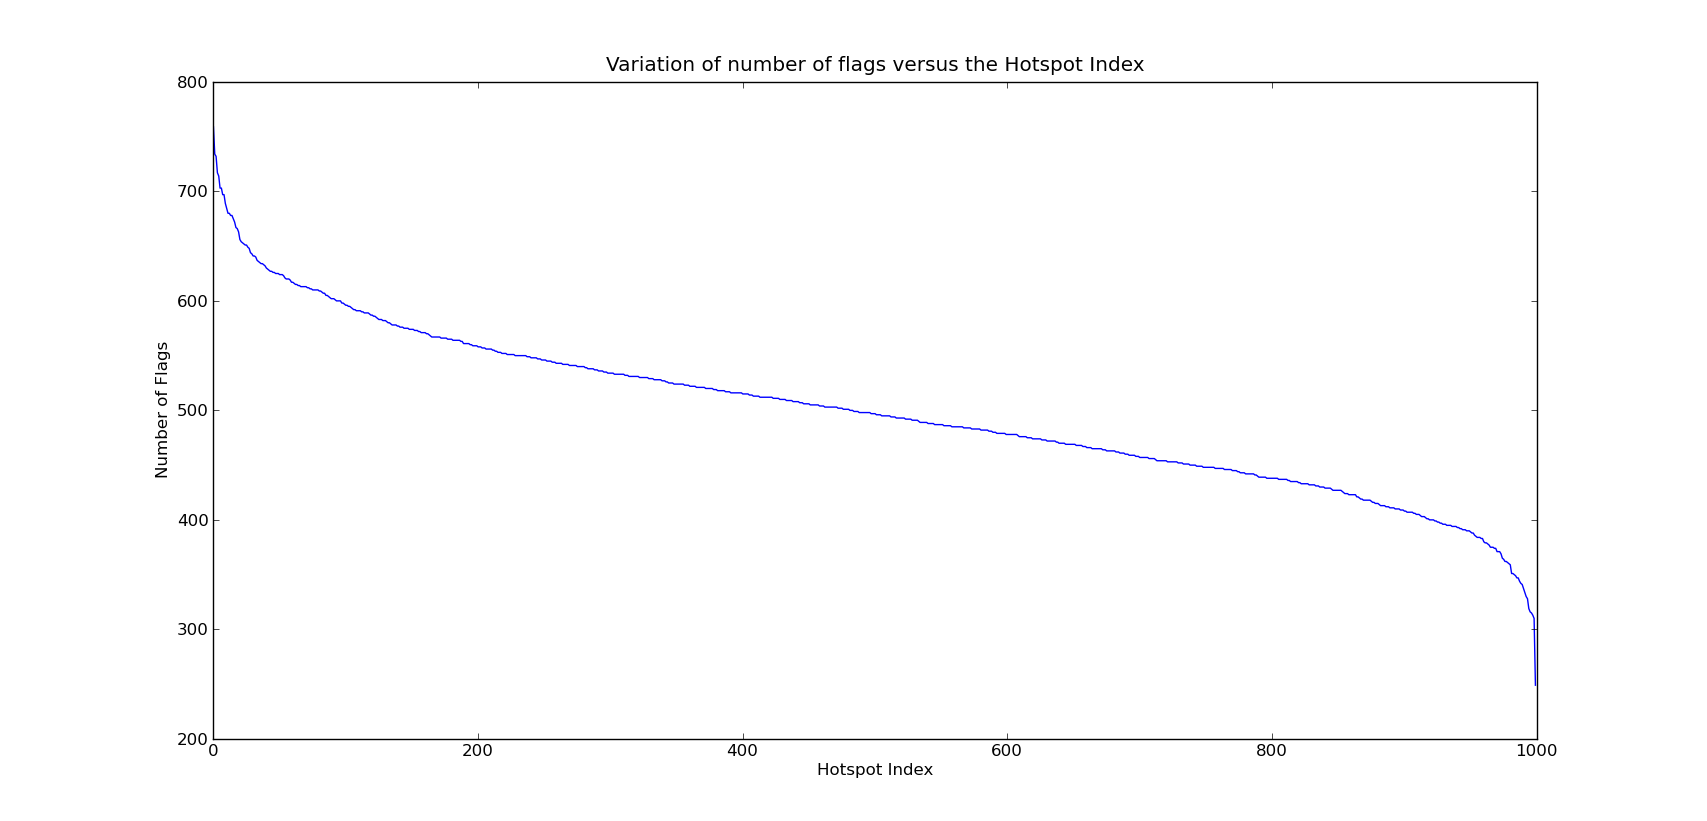
\includegraphics[scale=0.2]{Results/ErdosRenyi100015cutpoint33.png}
\caption{Plot of variation of number of flags versus $HotSpotIndex$ 
for an Erdos-Renyi network of 1000 vertices and edge probability of 0.15.
\newline
$\alpha = 33$}
\label{4_optimum_er}
\end{figure}

\begin{figure}[h]
\centering
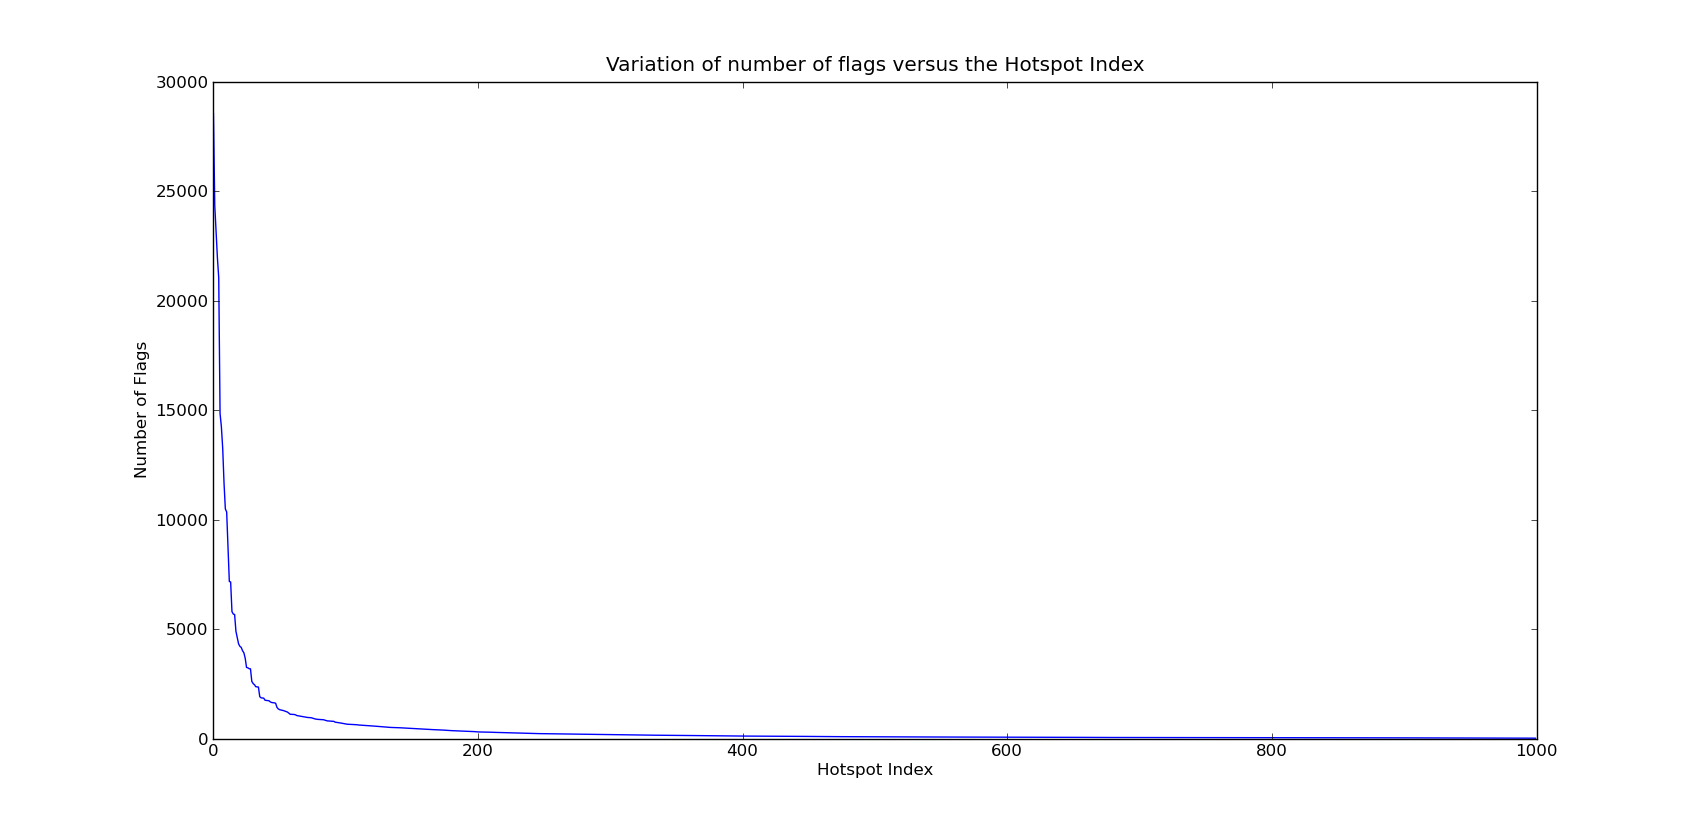
\includegraphics[scale=0.2]{Results/scalefreenetworks10004cutpoint100.png}
\caption{Plot of variation of number of flags versus $HotSpotIndex$ for 
a Scale Free Graph of 1000 vertices and 4 connections.
\newline
$\alpha = 100$}
\label{4_optimum_ba}
\end{figure}

The $HotSpotOrdering$ list contains the vertex labels arranged in the 
decreasing order of their number of flags. Let $HotSpotIndex(u)$
denote the position of $u$ in $HotSpotOrdering$.\\
Let $HotSpotOrdering = \{h_1, h_2, h_3,.. h_{|V|}\}$.\\
Now, $HotSpotIndex(h_i)=i$. The plots in Figure~\ref{4_optimum_er} and~\ref{4_optimum_ba} represent the variation of $flag$ values v/s $HotSpotIndex$.\\

Let $\alpha = |HotSpots|$. As $\alpha$ decreases, the navigation through 
the network during the navigation phase (Section.~\ref{sec:4_navigation_phase}) becomes increasingly difficult since it takes a longer path to reach vertices in $HotSpots$. As $\alpha$ increases, the difficulty involved in computing the all pairs shortest path between the elements of $HotSpots$ using Djikstra's Algorithm increases cubically, $O(\alpha^3)$. Thus, there is a need to determine an optimal value for $\alpha$.\\

By analyzing the plot of number of flags versus $HotSpotIndex$, we see that the rate of decrease of flagging decreases drastically at the point where the curve takes a sharp turn. Further addition of vertices into $HotSpots$ doesn't contribute significantly towards improving the efficiency of our algorithm. In fact, it causes a computational overhead during the creation of $HotSpotLookup$. Hence, we set $\alpha$ to a value of the curve at which it takes a sharp turn (i.e. a drastic slope change value).\\

\subsection{Comparison Between Various Navigation Techniques}

This section highlights the effectiveness of greedy navigation over other methods of navigation. Let $s \in V$ be the source and $t \in V$ be the target vertex. 
%In the navigation phase of the algorithm, our aim is to establish a path between $s$ and $t$. 
Let $d(s,t)$ denote the length of the shortest path between $s$ and $t$. Here are a few methods one can adopt to accomplish the task of establishing a path between $s$ and $t$:\\

\subsubsection {1-Way Random Walk}
The idea here is to start from the source vertex $s$ and take a random walk  $W_s$ until the target vertex $t$ is reached. Since this technique involves  a single random walk, we refer to it as a 1-way random walk. Let $\beta_{s,t}$ denote the path length of the path corresponding to the random walk $W_s$ from $s$ to $t$. Let $\beta$ be the average ratio of length of 1-way random walk and length of the shortest path, taken over all unordered vertex pairs $(s,t)$, such that $s,t \in V$.$$\beta = \frac{1}{\left(\begin{array}{c} |V|\\ 2\end{array}\right)} \sum_{s,t \in V} 
\frac{\beta_{s,t}}{d(s,t)}$$

% Figure.~\ref{4_one_way} illustrates the technique of 1-way random walk from $s$ to $t$. $W_s$ terminates when it reaches $t$. $W_s$ is indicated by the red walk. The source $s$ and target $t$ is denoted by the red dots. The blue dots indicate the other vertices in the network.\\
% 
% \begin{figure}[htp]
% \centering
% 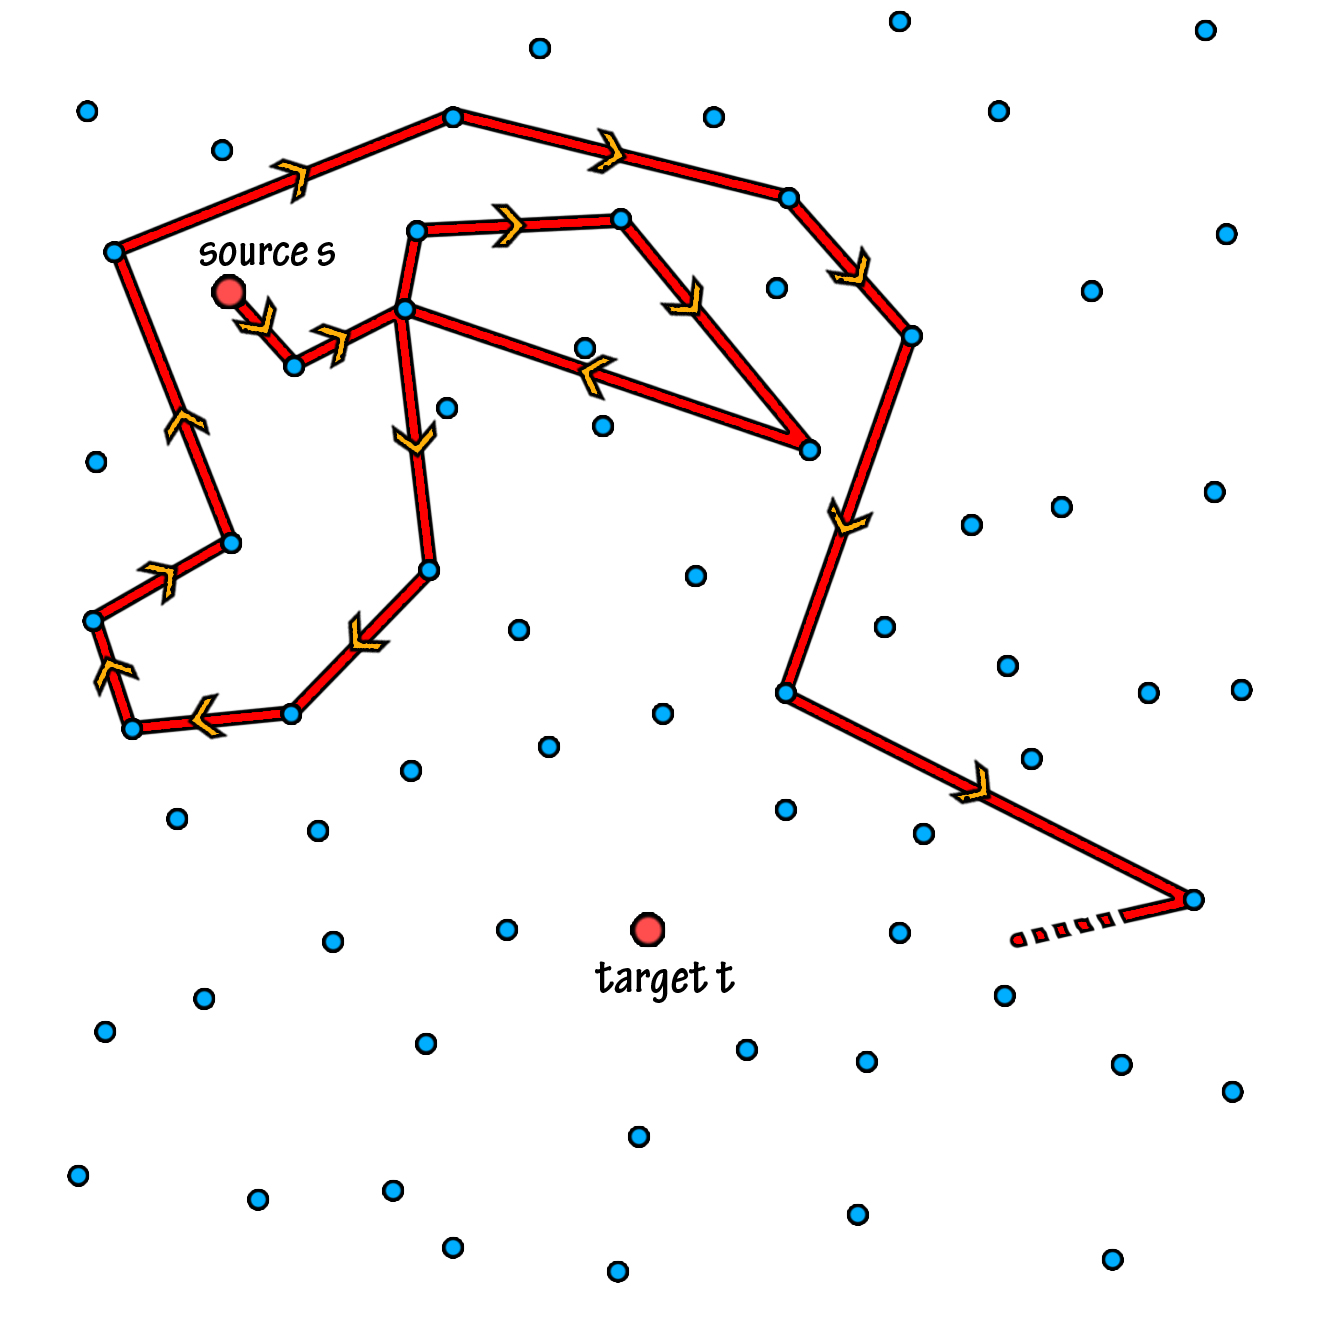
\includegraphics[scale=0.14]{Results/1rawrandomwalk.jpg}
% \caption{1-way Random Walk}
% \label{4_one_way}
% \end{figure}

\subsubsection{2-Way Random Walk}

After taking random walks $W_s$ and $W_t$ from $s$ and $t$ simultaneously 
until the two walks intersect, one can find a path from $s$ to $t$. Let $\gamma_{s,t}$ denote the length of the path thus obtained. $\gamma$ is defined on similar lines with $\beta$, as follows:
%Let $\gamma$ be the average ratio of length of 2-way Random Walk and the length of the shortest path taken over all the unordered vertex pairs $(s,t)$, such that $s,t \in V$.\\

$$\gamma = \frac{1}{\left(\begin{array}{c} |V|\\ 2\end{array}\right)} \sum_{s,t \in V} \frac{\gamma_{s,t}}{d(s,t)}$$

% Figure~\ref{4_two_way} illustrates the technique of 2-way random walk between $s$ and $t$. $W_s$ and $W_t$ are constructed simultaneously until they intersect. The intersection point of the two walks is indicated by $H$. $W_s$ and $W_t$ are indicated by the red walk and green walk respectively. Source $s$ and the target $t$ are denoted by the red dots.\\
% 
% \begin{figure}[htp]
% \centering
% 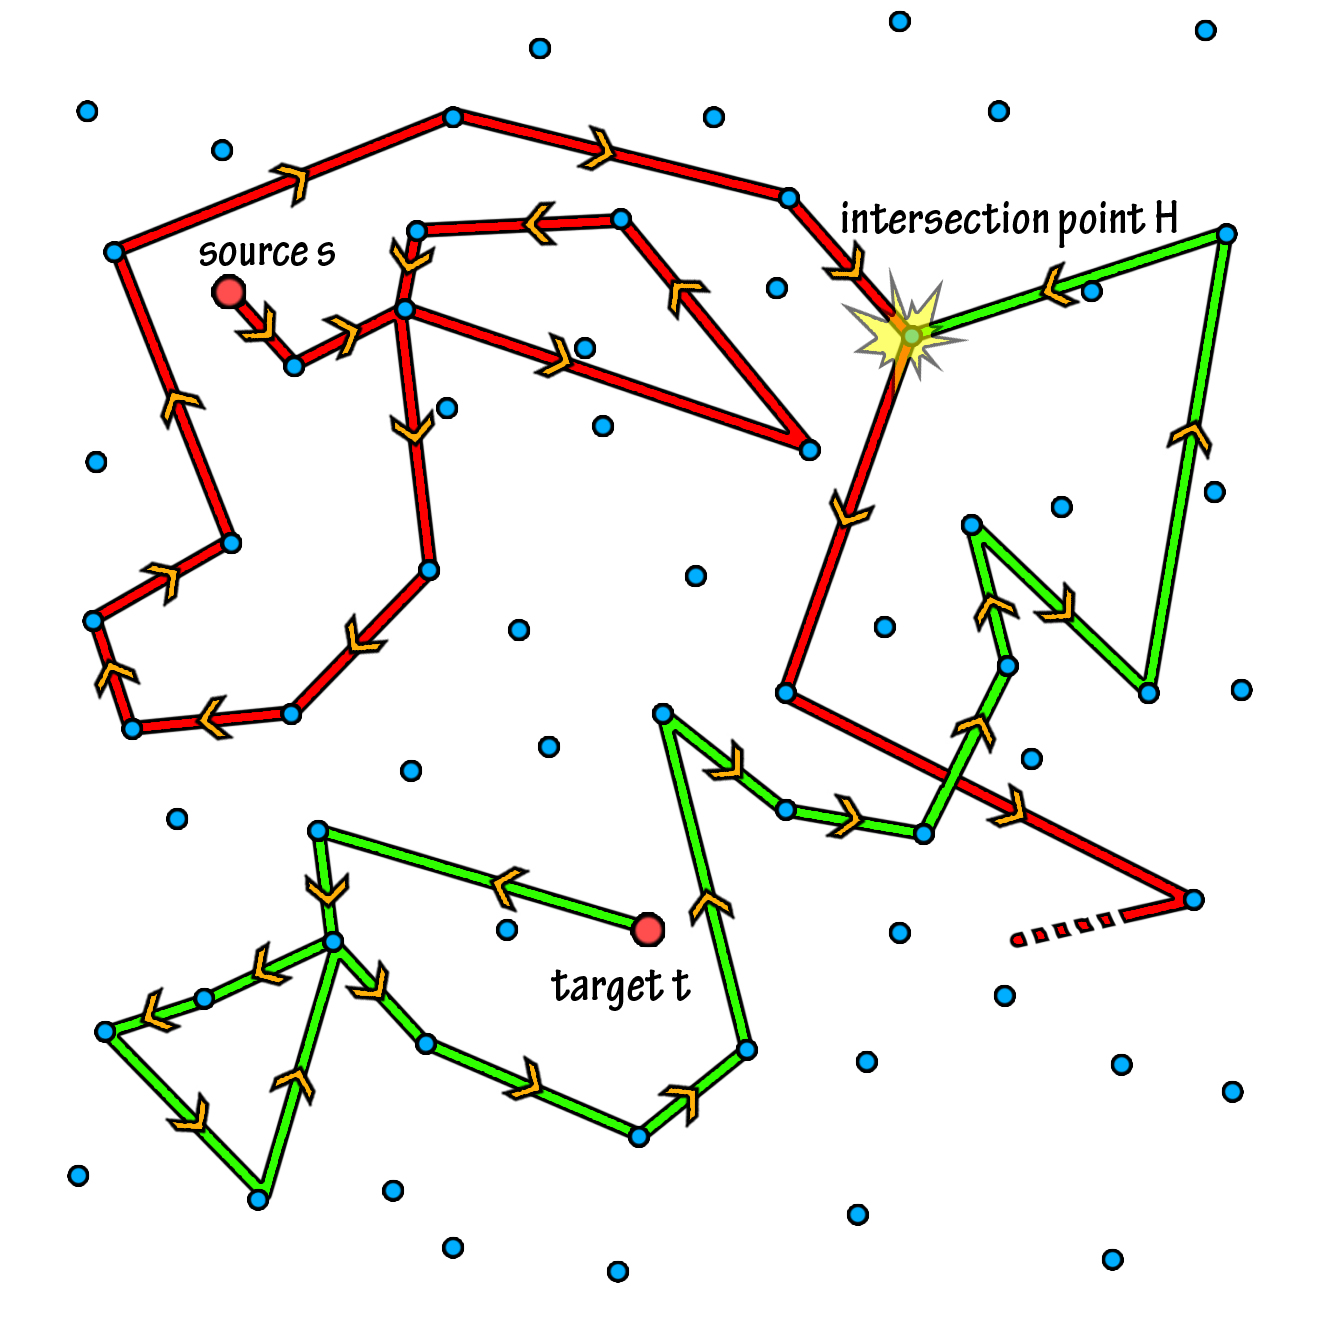
\includegraphics[scale=0.15]{Results/2rawrandomwalk.jpg}
% \caption{2-Way Random Walk}
% \label{4_two_way}
% \end{figure}

\subsubsection{Path Concatenation Algorithm}
Let $\delta_{s,t}$ denote the length of the path from $s$ to $t$ obtained after executing the path concatenation algorithm. $\delta$ is also defined on similar lines with $\beta$, as folows:

%Let $\delta$ be the average ratio of length of the path obtained by the path concatenation algorithm and the length of the shortest path, taken over all the unordered vertex pairs $(s,t)$, such that $s,t \in V$.

$$\delta = \frac{1}{\left(\begin{array}{c} |V|\\ 2\end{array}\right)} 
\sum_{s,t \in V(G)} \frac{\delta_{s,t}}{d(s,t)}$$

\begin{figure}[htp!]
\centering
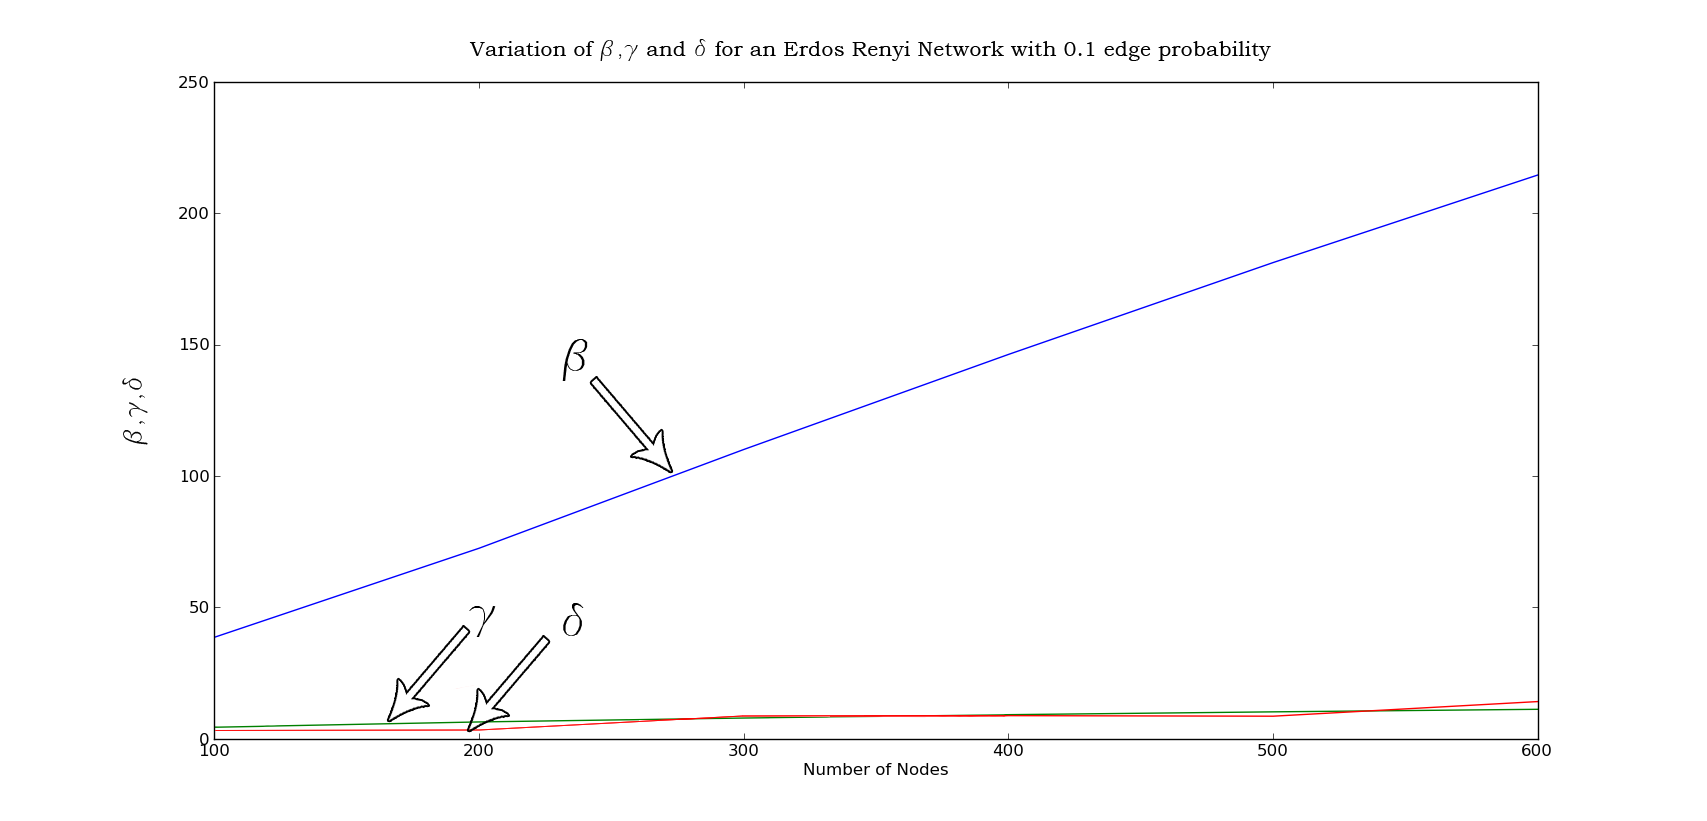
\includegraphics[scale=0.2]{Results/WalkComparisonErdos10.png}
\caption{Plot of $\beta$, $\gamma$ and $\delta$ 
versus the number of vertices for an Erdos-Renyi network with an edge probability of 0.1}
\label{4_performance_er}
\end{figure}

\begin{figure}[htp!]
\centering
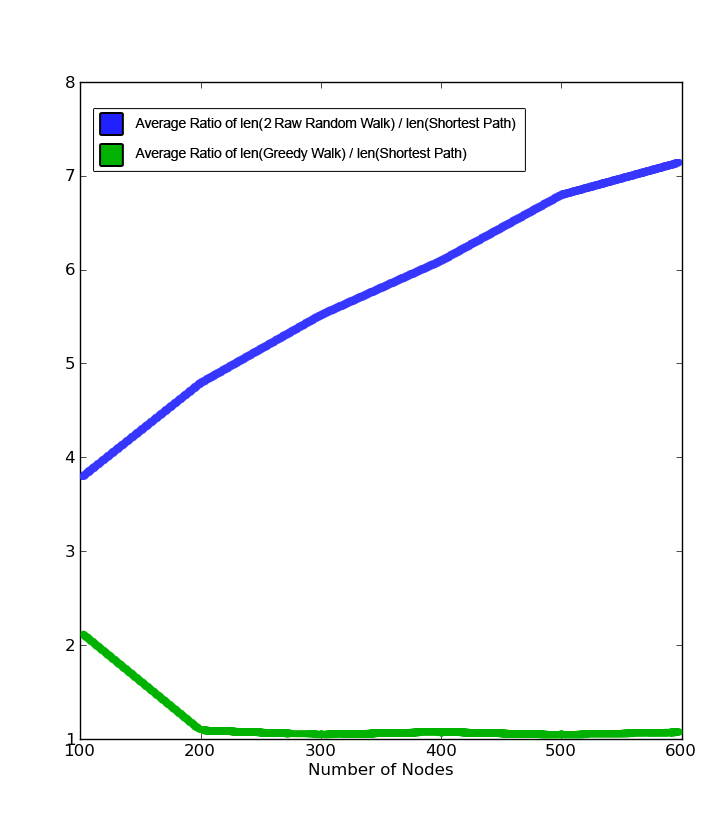
\includegraphics[width=.19\textheight]{Results/barabasi4connections2raw.jpg}
\caption{Plot of $\gamma$ (blue curve) and $\delta$ (green curve) versus the number of vertices for a Scale-free Graph with 4 connections}
\label{4_performance_ba_zoom}
\end{figure}


Figure.~\ref{4_performance_er} is a plot of variation of $\beta$, $\gamma$ and $\delta$ versus the number of vertices for an Erdos-Renyi network with an edge probability of 0.1. From the plot, it is clear that the $\delta$-curve always lies below the $\beta$ curve. This implies that, the greedy navigation performs better than 1-way Random Walk.\\

In case of Erdos-Renyi networks, the $\delta$ curve and the $\gamma$ curve lie very close to each other, and also intersect at certain points in the plot. Hence, the performance of PCA is as good as a 2-way random walk technique.\\

From Figure~\ref{4_performance_ba_zoom}, it is evident that in case the of scale-free graphs, the $\delta$ curve always lies below that of the $\gamma$ curve. Hence, the performance of PCA is better than that of the 2-way random walk technique.\\

\subsection{Hotspot Distribution for Erdos-Renyi and Scale-free graphs}

The hotspot set we introduced exhibit some characteristic features. In the case of Erdos-Renyi graphs, we note that the PCA doesn't perform significantly better than the 2-way random walk. The reason being that the Erdos-Renyi graphs do not contain vertices of relatively high degree. Whereas in case of a scale-free graph, some vertices have very high degree (\emph{hubs}) while the rest have relatively low degree. These \emph{hubs} form valid candidates for the hotspot set. They can be reached in a few hops from any vertex in the graph, thus making the PCA an efficient strategy.

\begin{figure}[htp]
\begin{center}
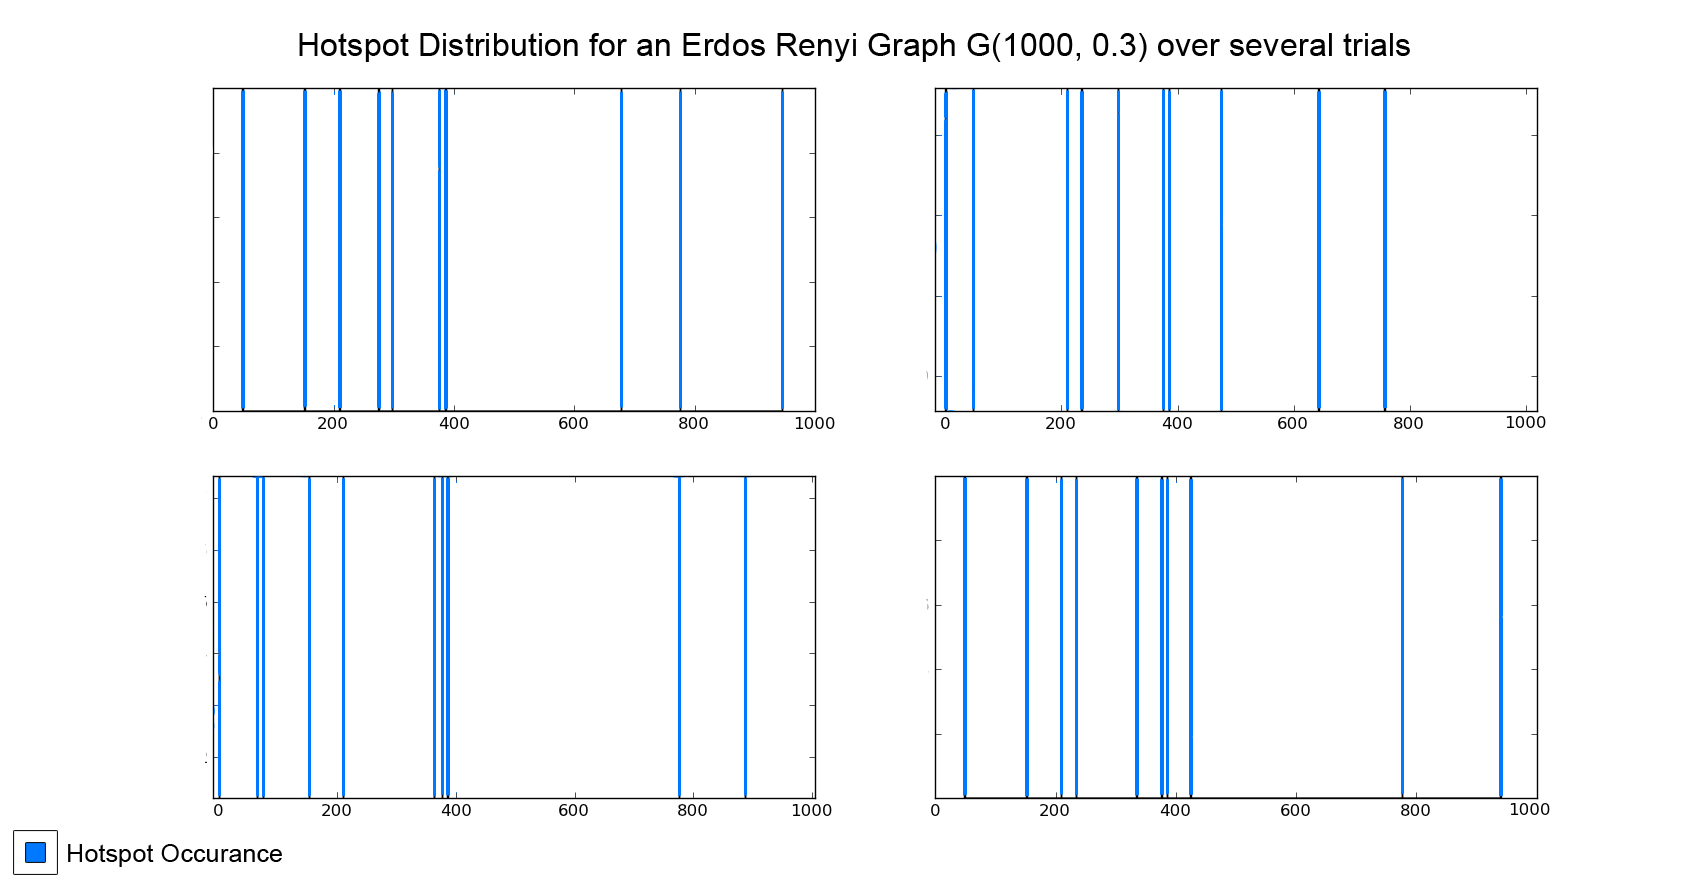
\includegraphics[scale=0.17]{Results/erdos.png}
\caption{Hotspot Distribution for an Erdos-Renyi Graph. x-axis represents the vertex name and the vertical lines represent the hotspots}
\label{4_hotspot_er}
\end{center}
\end{figure}

\begin{figure}[htp]
\begin{center}
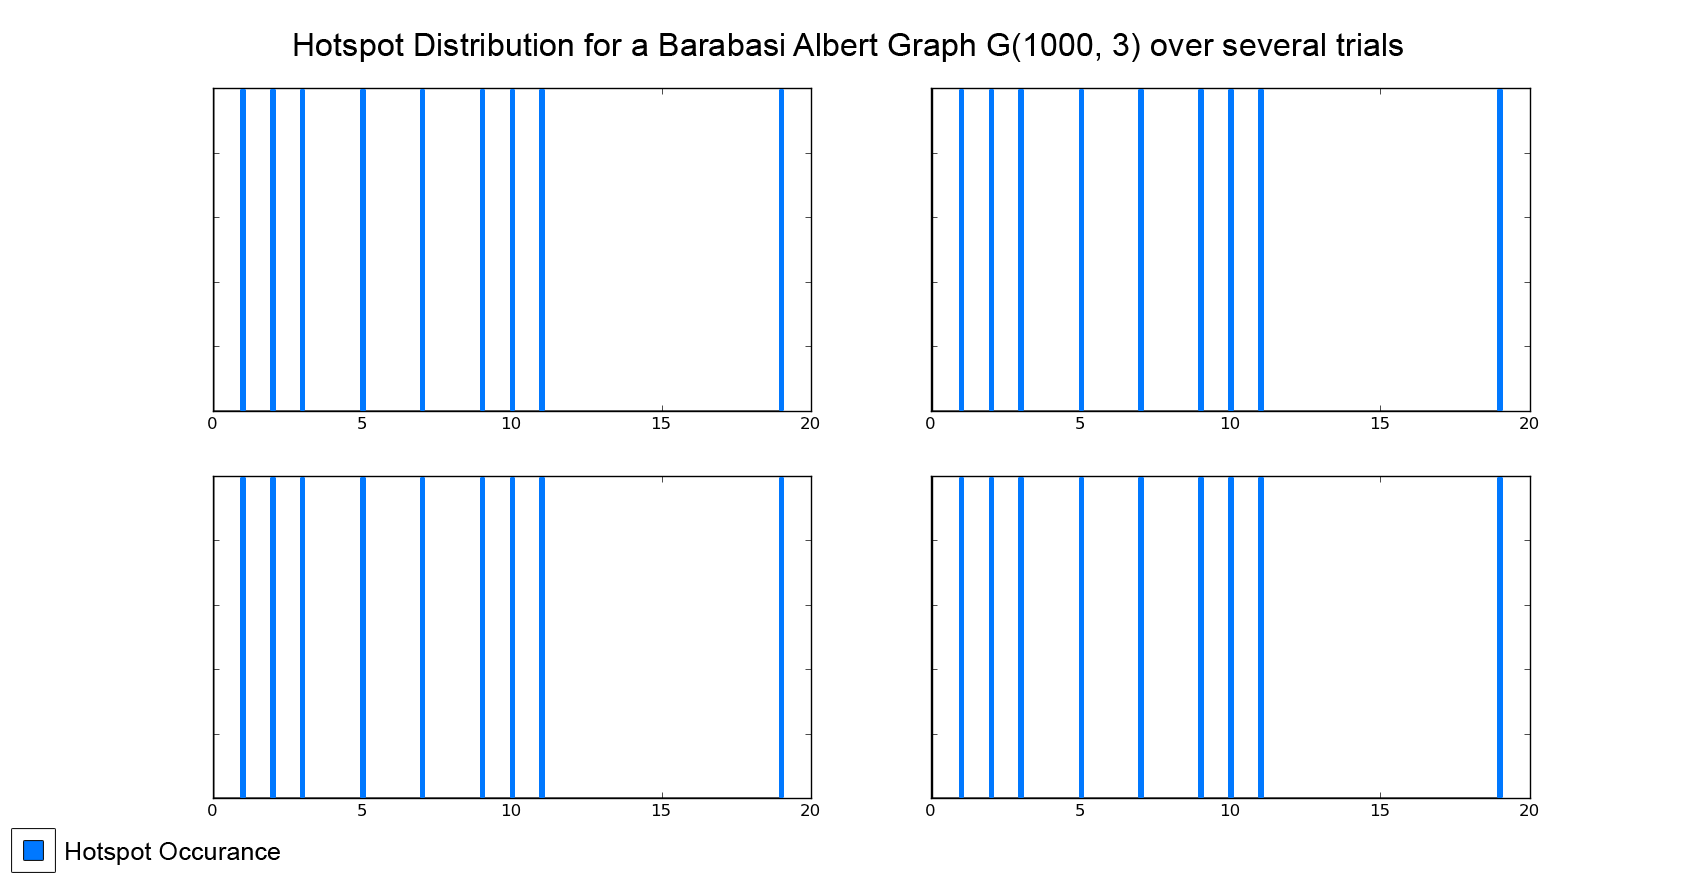
\includegraphics[scale=0.17]{Results/barabasi.png}\\
\caption{Hotspot Distribution for a Scale-free Graph. x-axis represents the vertex name and the vertical lines represent the hotspots}
\label{4_hotspot_ba}
\end{center}
\end{figure}

Fixing an Erdos-Renyi graph $G$ on 1000 vertices with probability $p=0.3$, as we run the learning phase of the PCA 4 times on the same graph, we note that the hotspot sets are different each time we run the algorithm. The top hotspot set is shown in Figure~\ref{4_hotspot_er}. E.g. if a vertex, say 306, has a vertical line, it means that the vertex is chosen as a hotspot. Repeating the same procedure on a scale-free graph, we note that the top hotspot set remains more or less the same as shown in Figure~\ref{4_hotspot_ba}.\\

\section{Center-strategic Paths on Scale Free Networks}

Given a path $(v_1,v_2,v_3,...,v_k)$ with closeness centrality values $(c_C(v_1),c_C(v_2),...,c_C(v_k))$ as defined in Section. \ref{sec:4_notions}, we compute the ranking of vertices $(R(v_1),R(v_2),R(v_3),...,R(v_k))$. By \emph{rank-plot} of this path, we mean a plot of the ranks $(R(v_1),R(v_2),R(v_3),...,R(v_k))$. If the rank-plot of a path has no more than one maxima, we call such a path a \emph{center-strategic path}.\\

The algorithm presented in this article is inspired by the strategy adapted by humans to learn the centers of a network and navigate in a center-strategic way. The presented algorithm resonates with the technique used by humans. We establish this fact by showing that the PCA algorithm yields center-strategic paths on scale free networks.

\begin{figure}[htp!]
\begin{center}
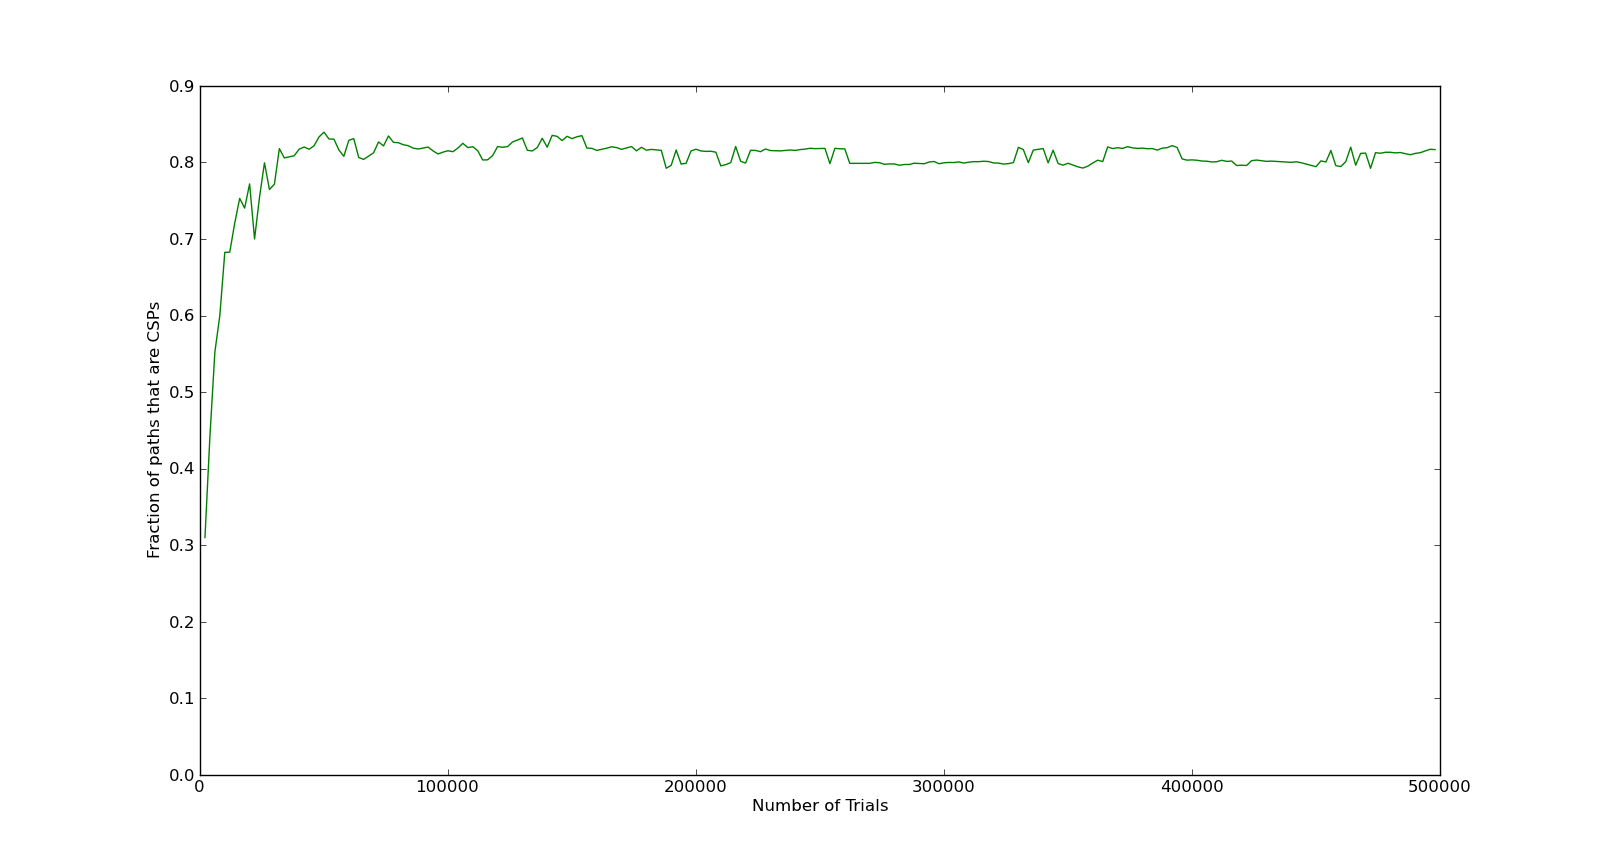
\includegraphics[width=.4\textheight]{Results/barabasi_csp.png}
\caption{Center Strategic Paths Using Path Concatenation Algorithm}
\label{4_mainplot}
\end{center}
\end{figure}

Consider a scale-free graph $G(V,E)$. Let $k$ denote the number of iterations (or trials) during the navigation phase of the path concatenation algorithm. After $k=100$, for every $k$, we jump to navigation phase, take $^{|V|}C_2$ greedy traversals (as explained in Section.~\ref{sec:4_navigation_phase}) between all vertex pairs and check for the number of paths that are center-strategic. The ratio of the number of center-strategic paths to the number of greedy traversals $^{|V|}C_2$ is denoted by $\psi$.\\

Figure.~\ref{4_mainplot} shows the variation of $\psi$ as k increases. We note that the path concatenation algorithm yields center-strategic paths 80\% of the times on scale free networks.\\

\section{Conclusion}
\label{sec:4_conclusion}

Motivated by the strategy adopted by humans to navigate in an unknown environment, we presented in this paper, an algorithm which simulates human navigation. We showed that the algorithm performs better than the 1-way and 2-way random walk technique. We further showed that the proposed algorithm generates center-strategic paths on scale-free networks.\\

A possible further work would be to study the convergence of the learning phase of the algorithm. One can start with the basic graph structures like the paths, grids, trees and study the hotspot distribution. It would also be interesting to classify the networks on which the algorithm performs well and those on which it does not. One can study the performance of PCA algorithm on real world networks as compared to other other navigational techniques.\\

% An example of a floating figure using the graphicx package.
% Note that \label must occur AFTER (or within) \caption.
% For figures, \caption should occur after the \includegraphics.
% Note that IEEEtran v1.7 and later has special internal code that
% is designed to preserve the operation of \label within \caption
% even when the captionsoff option is in effect. However, because
% of issues like this, it may be the safest practice to put all your
% \label just after \caption rather than within \caption{}.
%
% Reminder: the "draftcls" or "draftclsnofoot", not "draft", class
% option should be used if it is desired that the figures are to be
% displayed while in draft mode.
%
%\begin{figure}[!t]
%\centering
%\includegraphics[width=2.5in]{myfigure}
% where an .eps filename suffix will be assumed under latex, 
% and a .pdf suffix will be assumed for pdflatex; or what has been declared
% via \DeclareGraphicsExtensions.
%\caption{Simulation Results}
%\label{fig_sim}
%\end{figure}

% Note that IEEE typically puts floats only at the top, even when this
% results in a large percentage of a column being occupied by floats.


% An example of a double column floating figure using two subfigures.
% (The subfig.sty package must be loaded for this to work.)
% The subfigure \label commands are set within each subfloat command, the
% \label for the overall figure must come after \caption.
% \hfil must be used as a separator to get equal spacing.
% The subfigure.sty package works much the same way, except \subfigure is
% used instead of \subfloat.
%
%\begin{figure*}[!t]
%\centerline{\subfloat[Case I]\includegraphics[width=2.5in]{subfigcase1}%
%\label{fig_first_case}}
%\hfil
%\subfloat[Case II]{\includegraphics[width=2.5in]{subfigcase2}%
%\label{fig_second_case}}}
%\caption{Simulation results}
%\label{fig_sim}
%\end{figure*}
%
% Note that often IEEE papers with subfigures do not employ subfigure
% captions (using the optional argument to \subfloat), but instead will
% reference/describe all of them (a), (b), etc., within the main caption.


% An example of a floating table. Note that, for IEEE style tables, the 
% \caption command should come BEFORE the table. Table text will default to
% \footnotesize as IEEE normally uses this smaller font for tables.
% The \label must come after \caption as always.
%
%\begin{table}[!t]
%% increase table row spacing, adjust to taste
%\renewcommand{\arraystretch}{1.3}
% if using array.sty, it might be a good idea to tweak the value of
% \extrarowheight as needed to properly center the text within the cells
%\caption{An Example of a Table}
%\label{table_example}
%\centering
%% Some packages, such as MDW tools, offer better commands for making tables
%% than the plain LaTeX2e tabular which is used here.
%\begin{tabular}{|c||c|}
%\hline
%One & Two\\
%\hline
%Three & Four\\
%\hline
%\end{tabular}
%\end{table}


% Note that IEEE does not put floats in the very first column - or typically
% anywhere on the first page for that matter. Also, in-text middle ("here")
% positioning is not used. Most IEEE journals/conferences use top floats
% exclusively. Note that, LaTeX2e, unlike IEEE journals/conferences, places
% footnotes above bottom floats. This can be corrected via the \fnbelowfloat
% command of the stfloats package.



%-----------------------\section{Conclusion}
%-----------------------The conclusion goes here. this is more of the conclusion

% conference papers do not normally have an appendix


% use section* for acknowledgement
%-----------------------\section*{Acknowledgment}

%-----------------------The authors would like to thank...
%-----------------------more thanks here


% trigger a \newpage just before the given reference
% number - used to balance the columns on the last page
% adjust value as needed - may need to be readjusted if
% the document is modified later
%\IEEEtriggeratref{8}
% The "triggered" command can be changed if desired:
%\IEEEtriggercmd{\enlargethispage{-5in}}

% references section

% can use a bibliography generated by BibTeX as a .bbl file
% BibTeX documentation can be easily obtained at:
% http://www.ctan.org/tex-archive/biblio/bibtex/contrib/doc/
% The IEEEtran BibTeX style support page is at:
% http://www.michaelshell.org/tex/ieeetran/bibtex/
%\bibliographystyle{IEEEtran}
% argument is your BibTeX string definitions and bibliography database(s)
%\bibliography{IEEEabrv,../bib/paper}
%
% <OR> manually copy in the resultant .bbl file
% set second argument of \begin to the number of references
% (used to reserve space for the reference number labels box)

%-----------------------\begin{thebibliography}{1}
%-----------------------\bibitem{IEEEhowto:kopka}
%-----------------------H.~Kopka and P.~W. Daly, \emph{A Guide to \LaTeX}, 3rd~ed.\hskip 1em plus
%-----------------------  0.5em minus 0.4em\relax Harlow, England: Addison-Wesley, 1999.
%-----------------------\end{thebibliography}


\bibliographystyle{plain}  
\bibliography{references}

% that's all folks
\end{document}


